\documentclass[10pt,twocolumn,letterpaper]{article}  % ICCV

\usepackage{iccv}
\usepackage{times}
\usepackage{epsfig}
%\usepackage{graphicx}
%\usepackage{amsmath}
%\usepackage{amssymb}

% *** language support
%\usepackage[UTF8]{ctex}
\usepackage{xeCJK}
%\usepackage{verbatim}  % comment environment

% *** MATH PACKAGES ***
\usepackage{amssymb}
\usepackage{amsmath}
\usepackage{amsthm}
% *** GRAPHICS RELATED PACKAGES ***
\usepackage{graphicx}
\usepackage{subfigure}
% *** ALIGNMENT PACKAGES ***
%\usepackage{algorithm}
%\usepackage{algpseudocode}
%\usepackage{fancyhdr}

% If you comment hyperref and then uncomment it, you should delete
% egpaper.aux before re-running latex.  (Or just hit 'q' on the first latex
% run, let it finish, and you should be clear).
\usepackage[breaklinks=true,colorlinks,bookmarks=false,backref=page]{hyperref}

\iccvfinalcopy % *** Uncomment this line for the final submission

\def\iccvPaperID{****} % *** Enter the ICCV Paper ID here
\def\httilde{\mbox{\tt\raisebox{-.5ex}{\symbol{126}}}}

% Pages are numbered in submission mode, and unnumbered in camera-ready
\ificcvfinal\pagestyle{empty}\fi

% correct bad hyphenation here
\hyphenation{op-tical net-works semi-conduc-tor}


\begin{document}
\date{}
%%%%%%%%% TITLE
\title{A survey and design of drone-based Traffic Monitoring System}

\author{Rongji Xun$^{1}$\\
	$^{1}$Tongji University\\
	{\tt\small 2230815@tongji.edu.cn, rongji.xun@gmail.com }
	\thanks{This is a course report for ``视频编码与视觉感知''}
	% For a paper whose authors are all at the same institution,
	% omit the following lines up until the closing ``}''.
% Additional authors and addresses can be added with ``\and'',
% just like the second author.
% To save space, use either the email address or home page, not both
}


% make the title area
\maketitle

%%%%%%%%% ABSTRACT
\begin{abstract}
	With the increasing constructions of city roads and highways, the surveillance ability provided by fixed-device on gantries becomes quite limited. In this case, drone-based monitoring system could boost the traffic surveillance ability in a more easy-deploying and location-flexible way. We firstly do some survey on current traffic monitoring systems. After that we arrange the related datasets, metrics and algorithms like MOT(multi object tracking), object detection methods. Most importantly, we present our design on traffic monitoring system and achieve quite a satisfying result on our collected video data. Our codes and models are available at \url{https://github.com/LokiXun/traffic_monitoring_system_survey_and_simple_design}
\end{abstract}


%%%%%%%%% BODY TEXT
\section{Introduction}
The continuous increase in number of motorized vehicles and the ever-increasing travel demands call for innovative and effective measures to be taken to tackle the challenges of high traffic volumes and congestion levels.\cite{khan2017uav} However, the existing infrastructure constrained by the fixed-device and location, could hardly cover all the scope in the city to have a general view of the city's traffic situation. For this purpose, deploying drones to monitor the traffic situation is a more flexible and efficient ways to solve the limited monitoring problems.

\begin{figure}[!t]
	\centering
	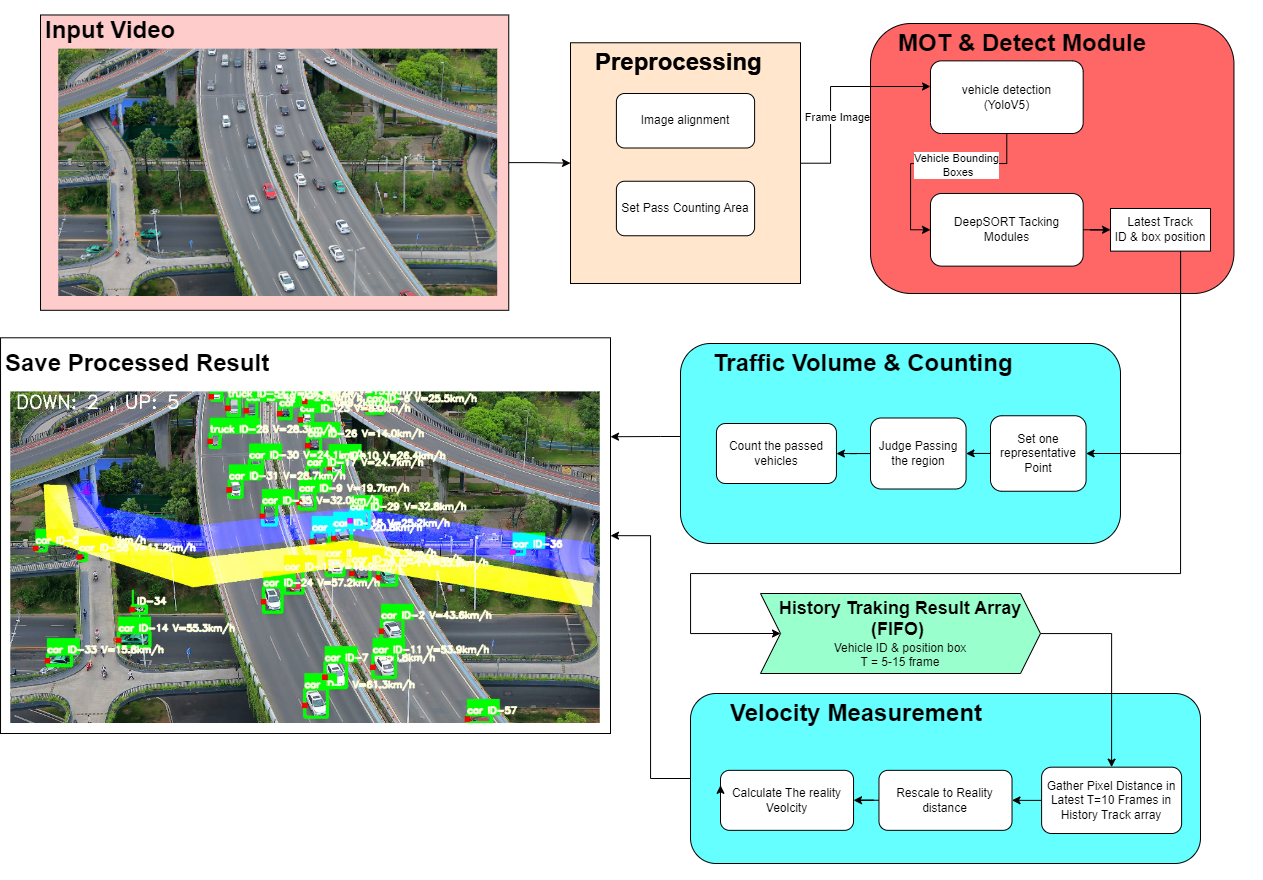
\includegraphics[width=0.95\linewidth]{./figures/traffic_monitoring_system_design.png} % requires the graphicx package
	\caption{Illustration of our Traffic Monitoring system framework. It incorporates MOT(Multi Object Tracking) methods to track cars in the video. The input videos are taken by drones and the drone could be steady in one position or moving with the object cars.}
	\label{fig:our-pipeline}
\end{figure}


There are some existing survey \cite{outay2020applications}, \cite{bisio2022systematic}, \cite{khan2017uav}, \cite{puri2005survey}, \cite{heintz2007images} of drone-based traffic monitoring system. Specially, \cite{bisio2022systematic} conduct a systematic review of drone-based traffic monitoring systems from a deep learning perspective. This work focuses on vehicle detection, tracking, and counting, since they are fundamental building blocks towards founding solutions for traffic congestion, flow rate and vehicle speed estimation. Additionally, drone-based datasets are examined, which face issues and problems caused by the diversity of features inherent of drone devices. The review analysis presented in \cite{bisio2022systematic} summarizes the literature solutions provided and deployed so far and discusses future research trends in establishing a comprehensive traffic monitoring system in support of the development of smart cities.

\cite{outay2020applications} presents a review of recent developments in relation to the application of UAVs in three major domains of transportation, namely; road safety, traffic monitoring and highway infrastructure management. Advances in computer vision algorithms to extract key features from UAV acquired videos and images are discussed along with the discussion on improvements made in traffic flow analysis methods, risk assessment and assistance in accident investigation and damage assessments for bridges and pavements. Additionally, barriers associated with the wide-scale deployment of UAVs technology are identified and countermeasures to overcome these barriers are discussed, along with their implications. 
\cite{puri2005survey} discusses and summarizes the research carried out all over the world until 2005 in the domain of UAV based traffic surveillance and analysis. \cite{heintz2007images} enlists and discusses the different modules of the proposed workflow i.e. flight planning, image acquisition and processing of UAV images. A particular focus is on the improvement of the UAV flight planning and control systems, eventually ensuring the quality of the acquired data. 


Unlike all existing surveys, we mainly focus on the overall framework of other drone-based monitoring system and also present our designed workflow by employing Deep learning based MOT(multi object Tracking) and object detection algorithms. To be more specific, as showed in Figure \ref{fig:our-pipeline}, we utilize YoloV5 \cite{github_yolov5} and DeepSORT \cite{wojke2017simple} in our project to detect and track the vehicles. The main contributions of this work are summarized as follows:
\begin{itemize}
	\item We categorize and summarize existing methods used in drone-based traffic monitoring system and make an in-depth and comprehensive survey on workflow design of drone-based traffic monitoring system. The summary provides insights for future algorithm design and new topic exploration.
	
	\item We summarize the widely used datasets and benchmark and analyze the approaches according to the object detection and tracking task in traffic monitoring system.
	
	\item We present our designed workflow illustrated in Figure \ref{fig:our-pipeline}, including vehicle velocity, volume measurement and density analysis sub-modules in traffic monitoring system.
\end{itemize}

The outline of this work is summarized as follows:

\tableofcontents
%\newpage




\section{Related Works}
In this section, we would discuss the related survey and works about traffic monitoring systems. \cite{jian2019combining} designs a general drone-based traffic congestion recognition workflow illustrated in Figure \ref{fig:jian2019combining_workflow}: images/videos acquisition, data processing and using CNN to make recognition result and send back to Traffic-Management Center.
\cite{khan2017uav} presents a detailed guide on implementing a UAV-based traffic monitoring system showed in Figure \ref{fig:khan2017uav_workflow}: firstly define the scope (decide the project objective, select the monitoring region like ramp or roadway segment and measure performance which is varied with the task like traffic volume, vehicle velocities). Then do the flight planning and dispatch the drones to take videos/images data. Finally analysis the data and optimize for defined task. In these schemes, the analyzing part in drone-based monitoring tasks can be done either on-board or via cloud-based processing.

\begin{figure}[!t]
	\centering
	\subfigure{\begin{minipage}[t]{1\linewidth}
		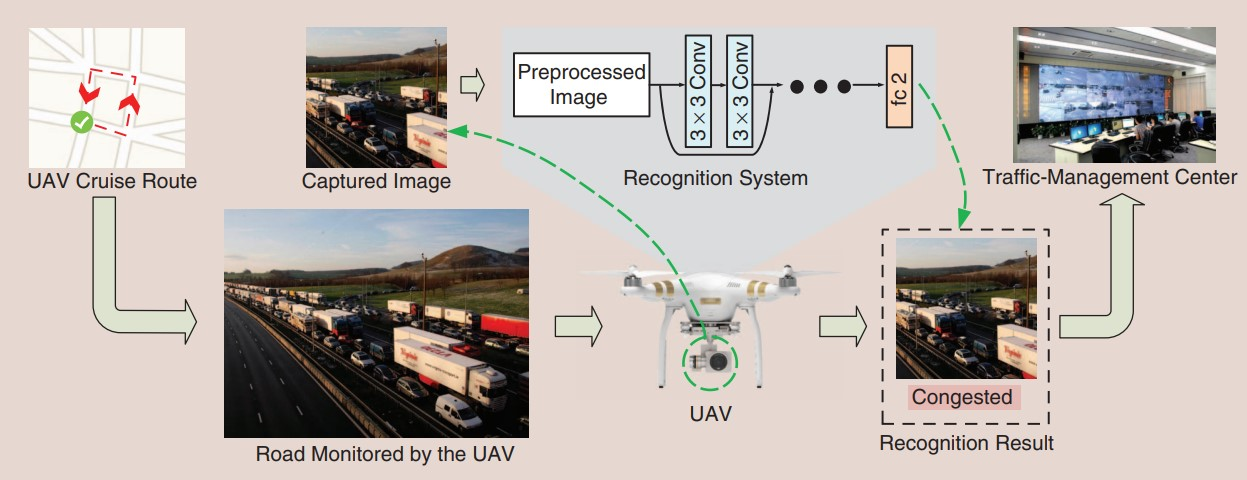
\includegraphics[width=0.95\linewidth]{./figures/Framework_in_Combining unmanned aerial vehicles with artificial-intelligence technology for traffic-congestion recognition.jpg} % requires the graphicx package
		\caption{A schematic used in \cite{jian2019combining} illustrating how a UAV-based traffic-congestion monitoring system works}
		\label{fig:jian2019combining_workflow}
	\end{minipage}}

	\subfigure{\begin{minipage}[t]{1\linewidth}
			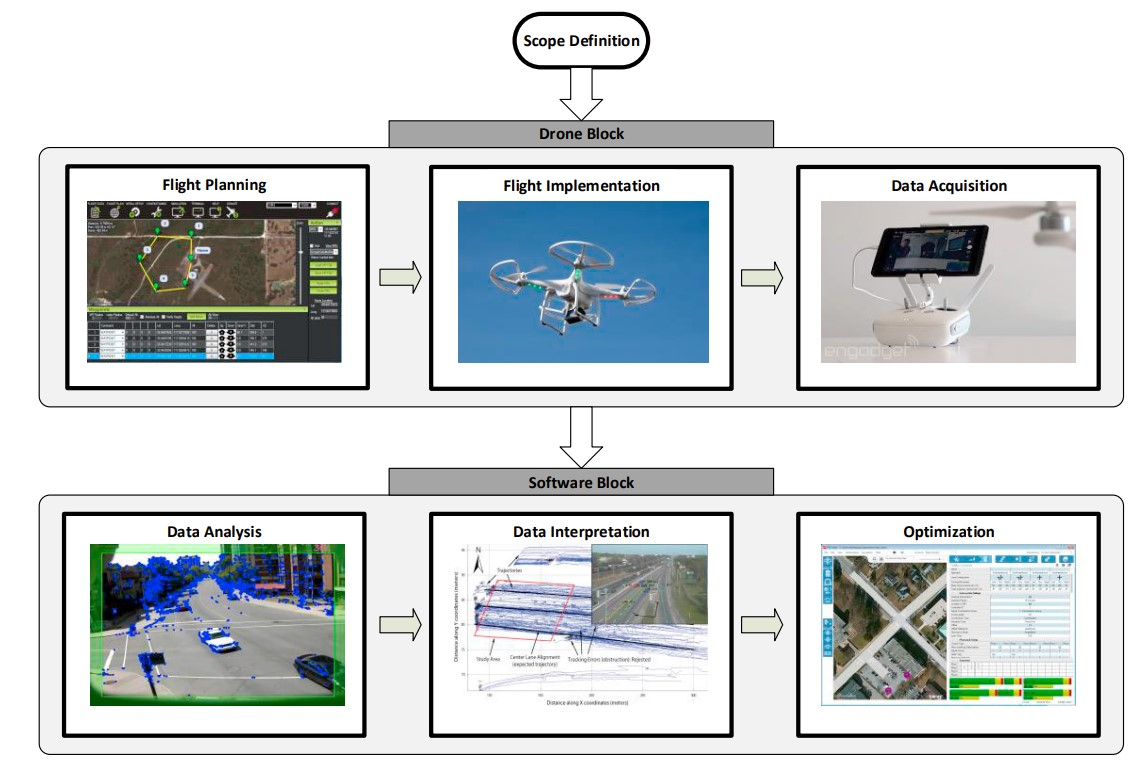
\includegraphics[width=0.95\linewidth]{./figures/khan2017uav_pipline.jpg} % requires the graphicx package
			\caption{A detailed workflow used by \cite{khan2017uav}, including scope definition, route planing, data processing part.}
			\label{fig:khan2017uav_workflow}
	\end{minipage}}
	\centering
	
\end{figure}

For the vehicle detection methods could be roughly split into two categories: 1) background segmentation: \cite{zhou2007moving} firstly divide image into small non-overlapped blocks and send the extracted PCA feature to SVM classifier judging whether the blocks belongs to any vehicle.  \cite{xu2016background} also employed a background subtraction technique and tested to be valid on various kind of scenes. 2) feature extraction based detection. Different object features, like Scale Invariant Feature Transformation (SIFT) used in \cite{mu2016multiple}, Haar-like features used in \cite{han2009vehicle}, and Histogram of oriented Gradients (HoG) are utilized in \cite{dalal2005histograms} to detect humans. 

In comparison, with the performance of Deep Learning methods soaring, some Deep Learning based works like \cite{li2019simultaneously}, \cite{zhu2018urban}, \cite{micheal2019automatic} are widely adopted.
% DL methods in traffic monitoring ---------------------




\section{Methodology}
\subsection{Multi Object Tracking}
MOT methods: Mean-shift, SORT, DeepSORT.
\subsubsection{Kalman Filter}
Kalman Filter
\subsubsection{Hungarian Algorithms}
Hungarian Algorithms

\subsection{Object Detection}
Faster-RCNN, YoloV1-V5, DETR.


\section{Traffic Datasets And Evaluating Metrics}
\subsection{Dataset}
Different from traditional image classification task, the traffics images that the drones acquired would have various shooting angles, high-density vehicles and tiny target size. These all resort to drones' shooting environment: 1)  wide angle camera make images contains high density vehicles; 2) moving drones and target objects contribute to image rotation, blurring problem; 3) tiny target size due to the high altitude.

To address the above issues, the availability of appropriate
datasets is a fundamental step towards finding suitable algorithmic solutions. In this connection, Convolutional Neural Networks (CNNs) are typically employed for image processing, and they are data hungry \cite{waqas2019isaid}.

In recent years, researchers have produced various drone-based aerial datasets to address data availability issues for different applications, which boost the development of drone-based vehicles detection and Tracking methods.\cite{bisio2022systematic}

The dataset presented in \cite{mueller2016benchmark} contains 110k frames to the purpose of object tracking from an aerial view. This dataset has been 285
acquired at low UAV altitude, with moving camera, and 286
different shooting angles, due to UAV motion \cite{bisio2022systematic}. Though \cite{mueller2016benchmark} lacks the data for dynamic weather and altitude settings, the moving camera and other features make it suitable for traffic monitoring task.

Visdrone \cite{zhu2021detection}, \cite{zhu2018vision}, the largest drone-based aerial datasets, which could be applied to four tasks: object detection in images or videos, object tracking like SOT and MOT. It includes 263 video sequences and more than 10000 static images, all of which were collected using various drones in 14 different cities in diverse weather and lighting conditions and 301
at various altitudes \cite{bisio2022systematic}.

Also, UAV Detection and Tracking (UAVDT) \cite{du2018unmanned} contains 80k images/Frames, with 1080$\times$540  resolutions, taken in 10-70m altitude with multiple camera-view. Mostly it is used for SOT(single object tracking) task. \cite{jensen2020presenting} proposed in 2020, an aerial dataset of a road scene is produced a static and a drone based camera, contains 4 object classes and 3.1k images in 1920$\times$ 1080 resolution and mainly used for traffic object detection task. Furthermore, Stanford Drone \cite{robicquet2016learning} includes six categories for objects. And the bicyclists, car and bus targets could be used for traffic surveillance task. 


\subsection{Object Tracking Task}
MOT metrics

\subsection{Object Detection Task}
object detection's metrics.



\section{Our System Framework}
\subsection{Our design}

\subsection{Traffic Velocity Measurement}
measure vehicles' veolcity.

\subsection{Traffic Flow Count And Density}
Constrained by the drones' limited view and the dynamic moving of vehicles, we assume to put drone be settled in the one place to overlook the road. In this setting, we count how many vehicle pass through the designated region for a period to calculate the traffic flow. 


For the Traffic Density, we simply calculate the number of vehicles had been detected in the valid regions and show on the System Graphic User Interface in real-time, which means the Traffic Density value would only be responsible for the current frame.
 
 
 \subsection{System Running Result}
 Show running result here.

\section{Limitations And Future Work}
Show experiment bad-case here.


\section{Conclusion}
In this work, we propose a our Traffic Monitoring System framework, in which YoloV5 and DeepSORT algorithms is applied to detect and track the vehicle in videos, which is taken by one moving drones. Extensive survey had been collected and analyzed.

\section*{Acknowledgment}
During this process of doing survey on related systems' paper, we learn lots of MOT, Object detection algorithms which might be helpful in our future research.


% references section
{\small
	\bibliographystyle{ieee_fullname}
	\bibliography{egbib}
}

\end{document}

